\documentclass[11pt]{article}
\usepackage[a4paper,margin=2.3cm]{geometry}
\usepackage[T1]{fontenc}
\usepackage[utf8]{inputenc}
\usepackage{newtxtext,newtxmath}
\usepackage{amsmath,graphicx,booktabs,makecell,enumitem,xcolor}
\usepackage[labelfont=bf]{caption}
\usepackage[hidelinks]{hyperref}
\usepackage{listings}
\renewcommand{\thetable}{S\arabic{table}}
\renewcommand{\thefigure}{S\arabic{figure}}
\renewcommand{\thesection}{S\arabic{section}}
\renewcommand{\theequation}{S\arabic{equation}}
\lstset{basicstyle=\ttfamily\small,frame=single,columns=fullflexible,breaklines=true}
% auto-generated by analysis/analyze.py -- do not edit
\newcommand{\RandomReturn}{8.85}
\newcommand{\RandomReturnSD}{2.71}
\newcommand{\RandomOnTimePct}{53.5}
\newcommand{\RandomWOnTimePct}{48.8}
\newcommand{\RandomComplPct}{67.8}
\newcommand{\RandomFatigue}{0.207}
\newcommand{\RandomAttention}{0.855}
\newcommand{\RandomBreakPct}{32.6}
\newcommand{\RandomHighFatPct}{0.0}
\newcommand{\FIFOReturn}{3.49}
\newcommand{\FIFOReturnSD}{3.49}
\newcommand{\FIFOOnTimePct}{43.2}
\newcommand{\FIFOWOnTimePct}{42.2}
\newcommand{\FIFOComplPct}{48.5}
\newcommand{\FIFOFatigue}{0.546}
\newcommand{\FIFOAttention}{0.463}
\newcommand{\FIFOBreakPct}{0.0}
\newcommand{\FIFOHighFatPct}{31.3}
\newcommand{\EDFReturn}{4.24}
\newcommand{\EDFReturnSD}{3.82}
\newcommand{\EDFOnTimePct}{46.8}
\newcommand{\EDFWOnTimePct}{45.4}
\newcommand{\EDFComplPct}{49.1}
\newcommand{\EDFFatigue}{0.545}
\newcommand{\EDFAttention}{0.465}
\newcommand{\EDFBreakPct}{0.0}
\newcommand{\EDFHighFatPct}{30.4}
\newcommand{\SPTReturn}{7.95}
\newcommand{\SPTReturnSD}{2.94}
\newcommand{\SPTOnTimePct}{62.5}
\newcommand{\SPTWOnTimePct}{49.4}
\newcommand{\SPTComplPct}{66.1}
\newcommand{\SPTFatigue}{0.477}
\newcommand{\SPTAttention}{0.543}
\newcommand{\SPTBreakPct}{0.0}
\newcommand{\SPTHighFatPct}{17.3}
\newcommand{\EDFPeriodicReturn}{11.41}
\newcommand{\EDFPeriodicReturnSD}{3.32}
\newcommand{\EDFPeriodicOnTimePct}{66.0}
\newcommand{\EDFPeriodicWOnTimePct}{65.7}
\newcommand{\EDFPeriodicComplPct}{74.1}
\newcommand{\EDFPeriodicFatigue}{0.296}
\newcommand{\EDFPeriodicAttention}{0.798}
\newcommand{\EDFPeriodicBreakPct}{18.8}
\newcommand{\EDFPeriodicHighFatPct}{0.0}
\newcommand{\EDFThresholdReturn}{11.35}
\newcommand{\EDFThresholdReturnSD}{3.28}
\newcommand{\EDFThresholdOnTimePct}{65.4}
\newcommand{\EDFThresholdWOnTimePct}{65.0}
\newcommand{\EDFThresholdComplPct}{74.2}
\newcommand{\EDFThresholdFatigue}{0.288}
\newcommand{\EDFThresholdAttention}{0.806}
\newcommand{\EDFThresholdBreakPct}{20.1}
\newcommand{\EDFThresholdHighFatPct}{0.0}
\newcommand{\CogHeuristicReturn}{10.59}
\newcommand{\CogHeuristicReturnSD}{2.76}
\newcommand{\CogHeuristicOnTimePct}{63.8}
\newcommand{\CogHeuristicWOnTimePct}{53.3}
\newcommand{\CogHeuristicComplPct}{78.0}
\newcommand{\CogHeuristicFatigue}{0.279}
\newcommand{\CogHeuristicAttention}{0.803}
\newcommand{\CogHeuristicBreakPct}{19.8}
\newcommand{\CogHeuristicHighFatPct}{0.0}
\newcommand{\DQNReturn}{10.66}
\newcommand{\DQNReturnSD}{0.33}
\newcommand{\DQNOnTimePct}{68.6}
\newcommand{\DQNWOnTimePct}{60.6}
\newcommand{\DQNComplPct}{73.2}
\newcommand{\DQNFatigue}{0.391}
\newcommand{\DQNAttention}{0.692}
\newcommand{\DQNBreakPct}{10.5}
\newcommand{\DQNHighFatPct}{0.2}
\newcommand{\AADQNReturn}{12.19}
\newcommand{\AADQNReturnSD}{0.27}
\newcommand{\AADQNOnTimePct}{72.6}
\newcommand{\AADQNWOnTimePct}{65.7}
\newcommand{\AADQNComplPct}{76.5}
\newcommand{\AADQNFatigue}{0.326}
\newcommand{\AADQNAttention}{0.761}
\newcommand{\AADQNBreakPct}{15.9}
\newcommand{\AADQNHighFatPct}{0.0}
\newcommand{\bestHeur}{EDF-Periodic}
\newcommand{\bestHeurReturn}{11.41}
\newcommand{\bestHeurOnTimePct}{66.0}
\newcommand{\bestHeurFatigue}{0.296}
\newcommand{\bestHeurBreakPct}{18.8}
\newcommand{\bestHeurAttention}{0.798}
\newcommand{\aaReturn}{12.19}
\newcommand{\aaReturnSD}{0.27}
\newcommand{\aaOnTimePct}{72.6}
\newcommand{\aaFatigue}{0.326}
\newcommand{\edfOnTimePct}{46.8}
\newcommand{\edfFatigue}{0.545}
\newcommand{\fatigueRedVsEdfPct}{40}
\newcommand{\onTimeGainVsEdfPP}{25.8}
\newcommand{\dRetRandom}{3.34}
\newcommand{\dRetRandomLo}{3.13}
\newcommand{\dRetRandomHi}{3.55}
\newcommand{\rbRetRandom}{0.97}
\newcommand{\winRetRandomPct}{92.8}
\newcommand{\seedsRetRandom}{10}
\newcommand{\dRetFIFO}{8.70}
\newcommand{\dRetFIFOLo}{8.47}
\newcommand{\dRetFIFOHi}{8.92}
\newcommand{\rbRetFIFO}{1.00}
\newcommand{\winRetFIFOPct}{99.8}
\newcommand{\seedsRetFIFO}{10}
\newcommand{\dRetEDF}{7.95}
\newcommand{\dRetEDFLo}{7.71}
\newcommand{\dRetEDFHi}{8.18}
\newcommand{\rbRetEDF}{1.00}
\newcommand{\winRetEDFPct}{100.0}
\newcommand{\seedsRetEDF}{10}
\newcommand{\dRetSPT}{4.24}
\newcommand{\dRetSPTLo}{4.06}
\newcommand{\dRetSPTHi}{4.41}
\newcommand{\rbRetSPT}{1.00}
\newcommand{\winRetSPTPct}{99.0}
\newcommand{\seedsRetSPT}{10}
\newcommand{\dRetEDFPeriodic}{0.77}
\newcommand{\dRetEDFPeriodicLo}{0.58}
\newcommand{\dRetEDFPeriodicHi}{0.95}
\newcommand{\rbRetEDFPeriodic}{0.34}
\newcommand{\winRetEDFPeriodicPct}{58.6}
\newcommand{\seedsRetEDFPeriodic}{10}
\newcommand{\dRetEDFThreshold}{0.84}
\newcommand{\dRetEDFThresholdLo}{0.66}
\newcommand{\dRetEDFThresholdHi}{1.02}
\newcommand{\rbRetEDFThreshold}{0.37}
\newcommand{\winRetEDFThresholdPct}{60.4}
\newcommand{\seedsRetEDFThreshold}{10}
\newcommand{\dRetCogHeuristic}{1.59}
\newcommand{\dRetCogHeuristicLo}{1.45}
\newcommand{\dRetCogHeuristicHi}{1.74}
\newcommand{\rbRetCogHeuristic}{0.83}
\newcommand{\winRetCogHeuristicPct}{81.6}
\newcommand{\seedsRetCogHeuristic}{10}
\newcommand{\dOnRandom}{19.1}
\newcommand{\dOnRandomLo}{18.2}
\newcommand{\dOnRandomHi}{20.2}
\newcommand{\rbOnRandom}{1.00}
\newcommand{\winOnRandomPct}{95.8}
\newcommand{\seedsOnRandom}{10}
\newcommand{\dOnFIFO}{29.4}
\newcommand{\dOnFIFOLo}{28.6}
\newcommand{\dOnFIFOHi}{30.3}
\newcommand{\rbOnFIFO}{1.00}
\newcommand{\winOnFIFOPct}{99.0}
\newcommand{\seedsOnFIFO}{10}
\newcommand{\dOnEDF}{25.8}
\newcommand{\dOnEDFLo}{24.9}
\newcommand{\dOnEDFHi}{26.7}
\newcommand{\rbOnEDF}{1.00}
\newcommand{\winOnEDFPct}{99.0}
\newcommand{\seedsOnEDF}{10}
\newcommand{\dOnSPT}{10.1}
\newcommand{\dOnSPTLo}{9.4}
\newcommand{\dOnSPTHi}{10.8}
\newcommand{\rbOnSPT}{0.93}
\newcommand{\winOnSPTPct}{88.2}
\newcommand{\seedsOnSPT}{10}
\newcommand{\dOnEDFPeriodic}{6.6}
\newcommand{\dOnEDFPeriodicLo}{5.7}
\newcommand{\dOnEDFPeriodicHi}{7.5}
\newcommand{\rbOnEDFPeriodic}{0.67}
\newcommand{\winOnEDFPeriodicPct}{67.0}
\newcommand{\seedsOnEDFPeriodic}{10}
\newcommand{\dOnEDFThreshold}{7.3}
\newcommand{\dOnEDFThresholdLo}{6.4}
\newcommand{\dOnEDFThresholdHi}{8.2}
\newcommand{\rbOnEDFThreshold}{0.71}
\newcommand{\winOnEDFThresholdPct}{68.0}
\newcommand{\seedsOnEDFThreshold}{10}
\newcommand{\dOnCogHeuristic}{8.8}
\newcommand{\dOnCogHeuristicLo}{8.2}
\newcommand{\dOnCogHeuristicHi}{9.4}
\newcommand{\rbOnCogHeuristic}{0.93}
\newcommand{\winOnCogHeuristicPct}{84.6}
\newcommand{\seedsOnCogHeuristic}{10}
\newcommand{\dFatRandom}{0.119}
\newcommand{\dFatRandomLo}{0.115}
\newcommand{\dFatRandomHi}{0.124}
\newcommand{\rbFatRandom}{1.00}
\newcommand{\winFatRandomPct}{98.8}
\newcommand{\seedsFatRandom}{10}
\newcommand{\dFatFIFO}{-0.220}
\newcommand{\dFatFIFOLo}{-0.225}
\newcommand{\dFatFIFOHi}{-0.215}
\newcommand{\rbFatFIFO}{-1.00}
\newcommand{\winFatFIFOPct}{0.0}
\newcommand{\seedsFatFIFO}{0}
\newcommand{\dFatEDF}{-0.219}
\newcommand{\dFatEDFLo}{-0.223}
\newcommand{\dFatEDFHi}{-0.214}
\newcommand{\rbFatEDF}{-1.00}
\newcommand{\winFatEDFPct}{0.0}
\newcommand{\seedsFatEDF}{0}
\newcommand{\dFatSPT}{-0.151}
\newcommand{\dFatSPTLo}{-0.155}
\newcommand{\dFatSPTHi}{-0.147}
\newcommand{\rbFatSPT}{-1.00}
\newcommand{\winFatSPTPct}{0.0}
\newcommand{\seedsFatSPT}{0}
\newcommand{\dFatEDFPeriodic}{0.030}
\newcommand{\dFatEDFPeriodicLo}{0.026}
\newcommand{\dFatEDFPeriodicHi}{0.033}
\newcommand{\rbFatEDFPeriodic}{0.68}
\newcommand{\winFatEDFPeriodicPct}{77.6}
\newcommand{\seedsFatEDFPeriodic}{10}
\newcommand{\dFatEDFThreshold}{0.038}
\newcommand{\dFatEDFThresholdLo}{0.036}
\newcommand{\dFatEDFThresholdHi}{0.041}
\newcommand{\rbFatEDFThreshold}{0.92}
\newcommand{\winFatEDFThresholdPct}{91.0}
\newcommand{\seedsFatEDFThreshold}{10}
\newcommand{\dFatCogHeuristic}{0.047}
\newcommand{\dFatCogHeuristicLo}{0.044}
\newcommand{\dFatCogHeuristicHi}{0.049}
\newcommand{\rbFatCogHeuristic}{0.98}
\newcommand{\winFatCogHeuristicPct}{94.8}
\newcommand{\seedsFatCogHeuristic}{10}
\newcommand{\dRetVsDqn}{1.53}
\newcommand{\dRetVsDqnLo}{1.46}
\newcommand{\dRetVsDqnHi}{1.60}
\newcommand{\winRetVsDqnPct}{98.4}
\newcommand{\ablFullDiff}{0.77}
\newcommand{\ablFullLo}{0.58}
\newcommand{\ablFullHi}{0.96}
\newcommand{\ablFullDiffOnPP}{6.6}
\newcommand{\ablFullDiffOnLo}{5.7}
\newcommand{\ablFullDiffOnHi}{7.5}
\newcommand{\ablFullRet}{12.19}
\newcommand{\ablFullOnPct}{72.6}
\newcommand{\ablFullBest}{EDF-Periodic}
\newcommand{\ablFullBestRet}{11.41}
\newcommand{\ablFullBestOnPct}{66.0}
\newcommand{\ablFullP}{<10^{-4}}
\newcommand{\ablFullPOn}{<10^{-4}}
\newcommand{\ablFullFatigue}{0.326}
\newcommand{\trainTimeAA}{474}
\newcommand{\trainTimeDQN}{410}
\newcommand{\inferUs}{101}
\newcommand{\DQNSelReturn}{10.66}
\newcommand{\DQNSelOnTimePct}{68.6}
\newcommand{\DQNBestEp}{950}
\newcommand{\DQNFinalReturn}{9.47}
\newcommand{\DQNFinalOnTimePct}{64.8}
\newcommand{\AADQNSelReturn}{12.19}
\newcommand{\AADQNSelOnTimePct}{72.6}
\newcommand{\AADQNBestEp}{1480}
\newcommand{\AADQNFinalReturn}{11.35}
\newcommand{\AADQNFinalOnTimePct}{70.6}

\title{\textbf{Supplementary Material}\\[4pt]\large Attention-aware task scheduling under partial observability of human cognitive state: a memory-augmented deep reinforcement learning approach}
\author{P.\,N. Bhargav Teja, Lanka Sree Chathurya, Rajay Vedaraj I.S.\thanks{Corresponding author: rajay@vit.ac.in}\\ Vellore Institute of Technology, Vellore 632014, Tamil Nadu, India}
\date{}
\begin{document}
\maketitle
\tableofcontents
\bigskip
\section{Complete simulator specification}\label{sec:s-spec}

\subsection{Episode timeline}
Each episode (workday) is generated from a single integer seed that fixes, through independent draws from one pseudo-random generator: the arrival slots, difficulties and slack of all tasks; the initial state $(H_0,F_0)$; the process-noise sequence $\xi_{0:T-1}$; and the observation-noise sequence $\epsilon_{0:T}$. Because the noise sequences are pre-drawn, two policies evaluated on the same seed experience the same exogenous randomness (common random numbers), and their outcomes differ only through their decisions. Within slot $t$:
\begin{enumerate}[label=\arabic*.]
\item Tasks with $a_i\le t$ become available.
\item The scheduler receives $o_t$ (main text, Eq.~6), computed from $A_t$, $F_t$ and $\epsilon_t$.
\item The action is mapped to a task (EDF within the chosen class, with a fallback to the other class) or to rest.
\item If working on task $i$: the remaining work is decreased by $\rho_t$ (Eq.~5); if it reaches zero, the task is completed at $t+1$ and the task reward is credited; $H$ and $F$ are updated with the work branch of Eqs.~(2)--(3). If resting: the rest branch is applied.
\item Process noise is added to $H$, and both states are clipped to $[0,1]$.
\item The cognitive reward $\mu A_{t+1}-\lambda F_{t+1}$ is added, and every unfinished task whose deadline equals $t+1$ incurs the miss penalty (once).
\end{enumerate}

\subsection{Productivity function}
Figure~\ref{fig:s-eff} shows the work rate $\rho=\rho_0A^{0.5+d}(1-\kappa F)$ for representative difficulties and fatigue levels. At $A=0.9$ and $F=0.1$, an easy task ($d=0.2$) proceeds at 0.88 units/slot and a hard task ($d=1$) at 0.81. At $A=0.4$ and $F=0.8$, the rates fall to 0.32 and 0.15, respectively. Hard work is thus disproportionately penalised in low-attention states, which creates the incentive to match task difficulty to cognitive state.

\begin{figure}[h]
\centering
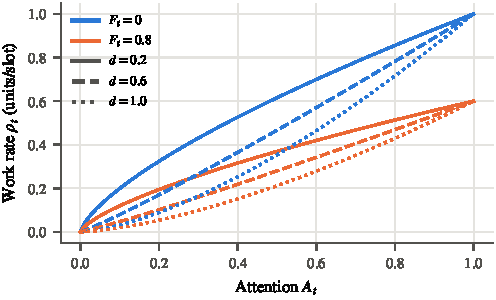
\includegraphics[width=0.55\textwidth]{figures/fig_efficiency.pdf}
\caption{Work rate as a function of attention for three difficulty levels and two fatigue levels.}
\label{fig:s-eff}
\end{figure}

\subsection{Environment variants used in the ablations}
\begin{itemize}
\item \textbf{No observation noise}: $\sigma_o=0$; the cognitive state is observed exactly (an MDP with respect to the cognitive variables, although future arrivals remain hidden).
\item \textbf{No circadian process}: $\gamma=0$, so that $A_t=H_t$.
\item \textbf{Static capacity (no cognition)}: $A_t\equiv0.60$ and $F_t\equiv0.30$ at all times. The resulting work rate of $0.60^{0.5+d}\times0.85$ (0.48 units/slot for $d=0.6$) delivers a daily throughput comparable to the break-taking heuristics in the full model, so the variant removes \emph{dynamics} without drastically changing \emph{capacity}. Breaks have no benefit in this variant.
\item \textbf{Task-only reward}: $\lambda=\mu=0$; the dynamics are unchanged.
\item \textbf{Worker profiles}: resilient ($\alpha,\delta\times0.7$; $\beta,\eta\times1.3$) and fatigue-prone ($\alpha,\delta\times1.3$; $\beta,\eta\times0.75$).
\item \textbf{Workload}: $N=8$ (4 initial) and $N=16$ (8 initial) tasks per day.
\end{itemize}

\section{Reproducibility}\label{sec:s-repro}
All experiments can be reproduced with the released code:
\begin{lstlisting}
pip install -r requirements.txt
python -m pytest                                 # simulator unit tests
python -m experiments.run_eval heuristics        # tune + test rule-based baselines
python -m experiments.run_rl --workers 4         # train all 107 agents
python -m experiments.run_eval robustness        # zero-shot robustness study
python -m experiments.run_eval traces            # behavioural traces
python -m analysis.analyze                       # all tables, figures, statistics
\end{lstlisting}
Seed ranges: training days $=s\times1\,000\,003+e$ for training seed $s$ and episode $e$; validation days $10^7,\dots,10^7+99$; test days $2\times10^7,\dots,2\times10^7+499$; tuning days $3\times10^7,\dots,3\times10^7+299$. One training run takes about \trainTimeAA{} s (AA-DQN) on a single CPU thread.


\section{Baseline tuning}\label{sec:s-tuning}
Table~\ref{tab:s-heur} lists the parameters selected by grid search for each environment variant (maximum mean return on 300 tuning days). ``off'' indicates that the fatigue threshold was never triggered ($\tau_F=1.01$). In the static-capacity variant, rest has no benefit, and all threshold rules learn to (almost) never rest.

\begin{table}[h]
\centering
\caption{Tuned heuristic parameters per environment variant.}
\label{tab:s-heur}
\small
\begin{tabular}{lccc}
\toprule
Variant & EDF-Periodic ($p$) & EDF-Threshold ($\tau_F,\tau_A$) & Cog-Heuristic ($\tau_F,\tau_A,\tau_H$) \\
\midrule
Full model & 4 & (0.6, 0.7) & (0.4, 0.6, 0.9) \\
No observation noise & 4 & (0.3, 0.7) & (0.3, 0.6, 0.9) \\
No circadian process & 4 & (0.4, 0.7) & (0.4, 0.6, 0.9) \\
Static capacity & 10 & (0.7, 0) & (0.7, 0, 0.8) \\
Task-only reward & 4 & (0.7, 0.7) & (0.5, 0.6, 0.9) \\
$\lambda=0.05$ & 4 & (0.6, 0.7) & (0.4, 0.6, 0.9) \\
$\lambda=0.2$ & 3 & (0.4, 0.7) & (0.3, 0.6, 0.9) \\
$\lambda=0.4$ & 2 & (0.3, 0.7) & (0.3, 0.6, 0.9) \\
\bottomrule
\end{tabular}
\end{table}

\section{Checkpoint selection}\label{sec:s-ckpt}
Table~\ref{tab:s-ckpt} compares, for each learned policy, the validation-selected checkpoint (primary results) with the final iterate after 5000 episodes. Selection improves both agents, which is consistent with the policy oscillation visible in Fig.~\ref{fig:s-train}. The ranking AA-DQN $>$ DQN holds for both checkpoint choices.

\begin{table}[h]
\centering
\caption{Test performance (500 days) of validation-selected versus final-iterate checkpoints (mean $\pm$ s.d.\ over ten seeds).}
\label{tab:s-ckpt}
\small
\begin{tabular}{llccc}
\toprule
Method & Checkpoint & Return & On-time rate & Mean selected episode \\
\midrule
DQN & validation-selected & 10.66 $\pm$ 0.33 & 0.686 $\pm$ 0.013 & 950 \\
DQN & final iterate & 9.47 $\pm$ 0.31 & 0.648 $\pm$ 0.009 & 3000 \\
AA-DQN & validation-selected & 12.19 $\pm$ 0.27 & 0.726 $\pm$ 0.009 & 1480 \\
AA-DQN & final iterate & 11.35 $\pm$ 0.41 & 0.706 $\pm$ 0.012 & 3000 \\
\bottomrule
\end{tabular}
\end{table}

\begin{figure}[h]
\centering
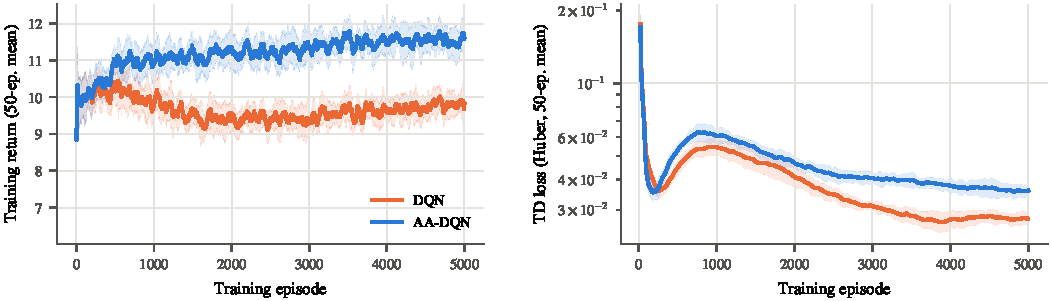
\includegraphics[width=\textwidth]{figures/fig_training_dynamics.pdf}
\caption{Training return (left; 50-episode moving average, $\epsilon$-greedy) and Huber TD loss (right) for DQN and AA-DQN (mean $\pm$ s.d.\ over ten seeds).}
\label{fig:s-train}
\end{figure}

\section{Component and sensitivity analysis}\label{sec:s-comp}
Table~\ref{tab:s-comp} reproduces the component study of the main text with all configurations, including the history length $k$ and the recurrent (GRU) encoder.

\begin{table}[h]
\centering
\caption{Component ablation and sensitivity (mean $\pm$ s.d.\ over seeds; 500 test days).}
\label{tab:s-comp}
\small
\resizebox{\textwidth}{!}{\begin{tabular}{lcccc}
\toprule
Configuration & Seeds & Return & On-time rate & Train time (s) \\
\midrule
AA-DQN (history $k{=}4$ + Double + Dueling) & 10 & 12.19 $\pm$ 0.27 & 0.726 $\pm$ 0.009 & 474 \\
Vanilla DQN ($k{=}1$, no Double/Dueling) & 10 & 10.66 $\pm$ 0.33 & 0.686 $\pm$ 0.013 & 410 \\
\bottomrule
\end{tabular}}
\end{table}

\section{Audit trail of the baseline set and action space}\label{sec:s-audit}
For transparency, we document a design change made during the study. In the first version of the experiments, the agent's action set contained only the intensity actions \{\textsc{easy}, \textsc{hard}, \textsc{break}\} of the original formulation, with EDF dispatch within the chosen class. The rule-based baselines were EDF-based (EDF-Periodic, EDF-Threshold, Cog-Heuristic). A pre-submission review argued that SPT-based rest heuristics should also be included, because SPT was the best classical rule in the static-capacity ablation. When added, SPT-Threshold obtained a higher test return than the intensity-only agent. The reason was structural: that agent could not express SPT sequencing. We therefore adopted the hybrid action set, in which every baseline is representable, added the observation of each class's shortest remaining work, set the training budget to 5000 episodes (the upper end of the range in our original protocol), and re-ran all experiments. To avoid over-fitting the design to the test set, this decision was made once, and no further design changes were made after the final runs were launched. The intensity-only agent trained under the final protocol is reported as a component ablation (Table~\ref{tab:s-comp}).

\section{Full robustness results}\label{sec:s-robust}
Table~\ref{tab:s-robust} reports the return and on-time rate of every method under each zero-shot test condition. Learned policies are averaged over training seeds, and heuristics use the parameters tuned in the nominal environment.

\begin{table}[h]
\centering
\caption{Zero-shot robustness: return / on-time rate on 500 test days per condition. Bold marks the best return.}
\label{tab:s-robust}
\small
\resizebox{\textwidth}{!}{\begin{tabular}{lcccccc}
\toprule
Test condition & AA-DQN & DQN & EDF-Periodic & EDF-Threshold & Cog-Heuristic & EDF \\
\midrule
$\sigma_o=0$ & \textbf{12.11 / 0.725} & 10.09 / 0.669 & 11.41 / 0.660 & 11.00 / 0.655 & 9.82 / 0.624 & 4.24 / 0.468 \\
Nominal ($\sigma_o=0.1$) & \textbf{12.19 / 0.726} & 10.66 / 0.686 & 11.41 / 0.660 & 11.35 / 0.654 & 10.59 / 0.638 & 4.24 / 0.468 \\
$\sigma_o=0.2$ & \textbf{12.32 / 0.728} & 11.22 / 0.701 & 11.41 / 0.660 & 10.77 / 0.615 & 10.01 / 0.587 & 4.24 / 0.468 \\
$\sigma_o=0.3$ & \textbf{12.40 / 0.725} & 11.66 / 0.711 & 11.41 / 0.660 & 9.63 / 0.557 & 8.04 / 0.482 & 4.24 / 0.468 \\
Resilient worker & 14.35 / 0.798 & 12.74 / 0.753 & \textbf{15.01 / 0.782} & 14.89 / 0.789 & 13.02 / 0.721 & 8.04 / 0.585 \\
Fatigue-prone worker & \textbf{10.10 / 0.655} & 8.72 / 0.620 & 7.46 / 0.529 & 7.91 / 0.521 & 8.72 / 0.579 & 1.43 / 0.382 \\
8 tasks/day & 11.85 / 0.931 & 8.94 / 0.816 & 13.06 / 0.973 & \textbf{13.12 / 0.974} & 12.51 / 0.934 & 6.84 / 0.723 \\
16 tasks/day & 9.00 / 0.505 & 9.09 / 0.518 & 7.32 / 0.417 & 7.02 / 0.405 & \textbf{9.30 / 0.509} & 1.70 / 0.331 \\
\bottomrule
\end{tabular}}
\end{table}

\section{Reward-weight sweep}\label{sec:s-pareto}
\begin{table}[h]
\centering
\caption{AA-DQN as a function of the fatigue weight $\lambda$ (attention weight $\mu=\lambda/2$; mean $\pm$ s.d.\ over three seeds).}
\label{tab:s-pareto}
\small
\begin{tabular}{cccccc}
\toprule
$\lambda$ ($\mu=\lambda/2$) & On-time rate & Mean fatigue & High-fatigue exposure & Break share \\
\midrule
0.1 & 0.725 $\pm$ 0.008 & 0.324 $\pm$ 0.013 & 0.000 & 0.163 \\
\bottomrule
\end{tabular}
\end{table}

\end{document}
